\newcommand{\gG}{\mathcal{G}\xspace}
\newcommand{\gL}{\mathcal{L}\xspace}
\newcommand{\gZ}{\mathcal{Z}\xspace}

\section{KG-guided LLM Enhancement}
LLMs have shown impressive communication and question-answering capabilities, demonstrating strong promise in various applications \cite{wang2024survey, wu2023bloomberggpt, cui2023chatlaw, chen2023genept, singhal2023large, singhal2023towards, haupt2023ai, nori2023capabilities, lee2023benefits, fleming2023assessing, chen2023meditron, yang2022large, luo2022biogpt, agrawal2022large, mehandru2024evaluating, zhang2023biomedgpt, biswas2023role, dash2023evaluation}. 
%answering medical questions \cite{singhal2023large, singhal2023towards, haupt2023ai, nori2023capabilities, lee2023benefits, fleming2023assessing, chen2023meditron}, extracting clinical information \cite{yang2022large, luo2022biogpt, agrawal2022large} and assisting clinical decisions \cite{mehandru2024evaluating, zhang2023biomedgpt, biswas2023role, dash2023evaluation}. 
%However, LLMs are also shown to ``hallucinate'' false outputs and unsubstantiated answers \cite{hal, hal3, hal4}, preventing their adoption in diverse fields, especially those with high-standard requirements on the accuracy and factuality of responses such as healthcare \cite{hal7}. Recently, many technical frameworks have been proposed to detect or avoid hallucinations in LLMs, such as based on supervision for reinforcement learning \cite{hal8}, statistical uncertainty measurements \cite{hal} and \todo{xxx \cite{}}. 
However, to reliably model domain-specific data and generate factual and accurate answers, LLMs still face the challenges of lacking domain knowledge, fuzzy inferences, and hallucination \cite{hu2023large, mousavi2024your, yadkori2024believe, asai2024selfrag,yu2024rankrag, liu2023evaluating, zhu2023dyval, zhuo2024roles, yuan2024back, wang2023boosting, ji2023survey, bai2024hallucination, tonmoy2024comprehensive, maynez2020faithfulness, xiao2021hallucination, farquhar2024detecting, ji2023towards, chen2024inside}.
% \textit{lack of knowledge} \cite{hu2023large, mousavi2024your, xu2024kg, becker2024cycles, yadkori2024believe, kim2024m}, \textit{fuzzy inference} \cite{liu2023evaluating, zhu2023dyval, bai2024kgquiz, zhuo2024roles, baek2024researchagent, yuan2024back, wang2023boosting}, and \textit{hallucination} \cite{ji2023survey, bai2024hallucination, tonmoy2024comprehensive, maynez2020faithfulness, xiao2021hallucination, farquhar2024detecting, ji2023towards, chen2024inside}
Retrieval augmented generation (RAG) \cite{lewis2020retrieval}, which aims at retrieving query-relevant evidence and generating evidence-based answers, has strong promise in evidence-critical domains. However, effective and efficient RAG for complex queries is still challenging which requires LLMs to be able to (1) generate logical plans for retrieving multiple pieces of relevant evidence from complex data, (2) conduct valid reasoning and inference to compose the pieces of evidence towards generating coherent answers, and (3) reliably guarantee the detection and removal of errors. In the following, we discuss how these challenges can be addressed with well-designed planning, reasoning, and reflection frameworks with the help of KGs.

{
\newcommand{\ourmethod}{\texttt{RoG}\xspace}
\subsection{Planning with domain knowledge}
% \carl{Linhao, the current 3.1 is too long-- we aim to write about 12 pages of main contents in total and the plan is to write about 2 (front page/intro)+ 3 (sec 2) + 3 (sec 3) + 2 (sec 4) + 1 (sec 5) + unlimited references. Can you perhaps try to separate the current contents into 3.1 (planning) and 3.2 (reasoning)? Please try to re-organize/re-write the contents more so they also read differently from your RoG paper. Please also add some discussions about more related recent works separately in both subsections. I added a reference in 3.3, but please let me know if you are not sure about what to write in 3.3. Thanks!}\\
While LLMs excel in many NLP tasks \cite{brown2020language,bang2023multitask}, they still face challenges in acquiring domain knowledge. To address this issue, many attempts seek assistance from KGs, which are often constructed to represent knowledge in specific domains, such as medicine \cite{bodenreider2004unified}, law \cite{kang2024bridging}, and finance \cite{liu2019anticipating}. The integration of KGs and LLMs has shown promising results in various applications, such as question answering \cite{jiang2023unikgqa}, recommendation \cite{wang2023enhancing}, and dialogue systems \cite{tuan2022towards}. Despite the success, there are still challenges in effectively obtaining useful information from KGs and incorporating them into LLMs. 

Existing methods typically depend on a retriever to obtain relevant triples. For example, Baek et al. \cite{baek2023direct} proposed a direct retrieval method to retrieve relevant triples from KGs. However, the retriever may not always retrieve the most relevant triples, leading to suboptimal performance. Additionally, KGs contain a wealth of domain-specific knowledge, making it challenging for LLMs with limited domain expertise to comprehend and utilize this information. To further unleash LLMs' capabilities of leveraging domain knowledge, the \textit{plan-and-solve} paradigm \cite{wang2023plan} has been proposed, in which LLMs are prompted to first generate a plan. Based on the plan, LLMs can retrieve the relevant domain knowledge and conduct reasoning to generate answers \cite{yaoreact}. However, existing methods are incapable of handling the complex structured knowledge in KGs to enable effective planning and reasoning. To address this issue, we propose a \textit{planning-retrieval-reasoning} framework named \ourmethod that enables LLMs to plan and reason on KGs \cite{luo2024reasoning}. The overall framework is illustrated in \Cref{fig:rog}.

\begin{figure}[htbp]
    \begin{center}
    %\framebox[4.0in]{$\;$}
    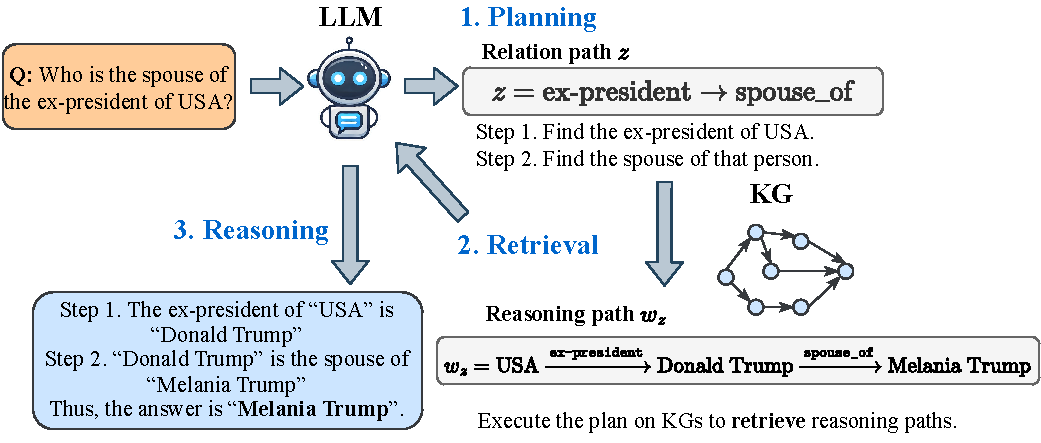
\includegraphics[width=.85\columnwidth]{submissions/CarlYang2024/figures/rog.pdf}
    \end{center}
    % \vspace{-3mm}
    \caption{The overall framework of planning and reasoning on KGs (\ourmethod).}
    \label{fig:rog}
    % \vspace{-5mm}
\end{figure}

\ourmethod first generates several relation paths that are grounded by KGs as plans. Relation paths, which capture semantic relations between entities, have been utilized in many reasoning tasks on KGs \cite{wang2021relational,xusubgraph}. Based on relation paths, we can always retrieve the latest knowledge from KGs with a simple constrained breadth-first search. Therefore, relation paths can serve as faithful plans to guide the retrieval and reasoning on domain-specific KGs. Additionally, by treating relation paths as plans, we can make sure the plans are grounded by KGs, which enables LLMs to retrieve relevant knowledge and conduct faithful reasoning. To this end, we formulate our \ourmethod as an optimization problem that aims to maximize the probability of reasoning the answer from a KG $\gG$ w.r.t the question $q$ by generating relation paths $z$ as the plan:
\begin{equation}
    % \setlength\abovedisplayskip{1pt}%shrink space
    % \setlength\belowdisplayskip{1pt}
    \label{eq:plan}
    P_\theta(a|q,\gG) = \sum_{z\in\gZ}P_\theta(a|q,z,\gG)P_\theta(z|q),
\end{equation}
where $\theta$ denotes the parameters of LLMs {and $a$ denotes the final answer.} To enable accurate planning with domain knowledge, we design two instruction tuning tasks: 1) \textit{planning optimization}, which distills the knowledge from KGs into LLMs to generate faithful relation paths as plans; 2) \textit{retrieval-reasoning optimization}, which enables LLMs to reason based on the retrieved reasoning paths.
{
The final objective function of \ourmethod is the combination of the planning optimization and retrieval-reasoning optimization, which can be formulated as
\begin{equation}
    \setlength\abovedisplayskip{1pt}%shrink space
    \setlength\belowdisplayskip{1pt}
    \label{eq:final_obj}
    \gL = \log \underbrace{P_\theta(a|q,\gZ^*_K,\gG)}_{\text{Retrieval-reasoning}} + \underbrace{\frac{1}{|\gZ^*|}\sum_{z\in Z^*}\log P_\theta(z|q)}_{\text{Planning}},
\end{equation}
where we use the shortest paths $\gZ^*\subseteq\mathcal{Z}$ between $q$ and $a$ in KGs as supervision signals. We maximize the probability of LLMs generating faithful relation paths through distilling the knowledge from KGs.
}
In this way, with the proposed \ourmethod, LLMs can effectively retrieve domain knowledge from KGs with planning, which significantly enhances the reasoning capability of LLMs.
}

{
    \newcommand{\ourmethod}{\texttt{GCR}\xspace}
\subsection{Reasoning with structured knowledge}
% https://arxiv.org/abs/2410.13080
KGs capture abundant factual knowledge in a structured format, which provides a faithful knowledge source for improving the reasoning abilities of LLMs \cite{pan2024unifying}. Nevertheless, because of the unstructured nature of LLMs, directly applying them to reason on structured KGs is challenging. Early works focus on fine-tuning LLMs together with structured knowledge from KGs to enrich the knowledge of LLMs for better reasoning \cite{zhang2019ernie,rosset2020knowledge}. For example, KEPLER~\cite{wang2021kepler} directly employs both KG embedding training objective and Masked token pre-training objective into a shared transformer-based encoder. Through fine-tuning, LLMs can better understand the structured knowledge in KGs for reasoning. However, the fine-tuning process is computationally expensive and incapable of efficiently adapting to the evolving real-world knowledge. 

Recently, researchers have combined the strengths of retrieval-based methods with the prompting technique to enable LLMs to reason on KGs \cite{lewis2020retrieval,jiang2023unikgqa}. CoK \cite{wang2023boosting} and KD-CoT \cite{wang2023knowledge} retrieve facts from an external KG to guide the CoT performed by LLMs. To capture graph structure, GNN-RAG \cite{mavromatis2024gnn} adopts a lightweight graph neural network to effectively retrieve knowledge from KGs, which are formatted as a sentence path to elicit the reasoning process of LLMs. Mindmap \cite{wen2023mindmap} builds a prompt-based method that endows LLMs with the capability of comprehending KG and reasoning with it. Despite the success of these methods, they still face challenges in designing principled prompts to represent KGs and conduct reasoning. Moreover, LLMs still have limited capabilities in understanding the graph structure and reasoning with the text-based graph prompts \cite{huang2024can}. 

Different from existing efforts that require a computationally expensive fine-tuning phase or design ad-hot prompts for LLMs,  we recently introduced a KG-constrained reasoning (\ourmethod) paradigm \cite{luo2024graph}. \ourmethod connects unstructured reasoning in LLMs with structured knowledge in KGs, seeking to achieve efficient and effective reasoning on structured knowledge. The overall framework is illustrated in \Cref{fig:gcr}.

\begin{figure}[htbp]
    \begin{center}
    %\framebox[4.0in]{$\;$}
    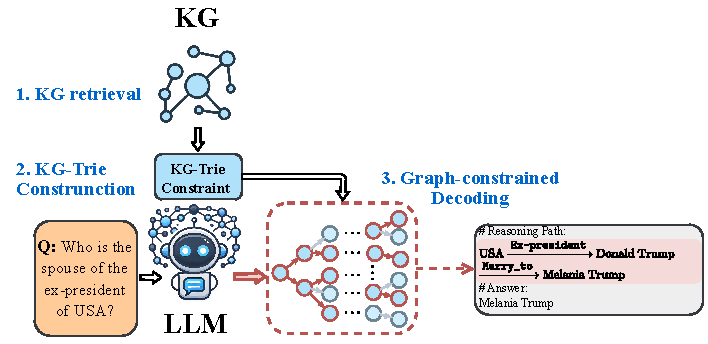
\includegraphics[width=.75\columnwidth]{submissions/CarlYang2024/figures/gcr.pdf}
    \end{center}
    % \vspace{-3mm}
    \caption{The overall framework of KG-constrained reasoning (\ourmethod).}
    \label{fig:gcr}
    % \vspace{-5mm}
\end{figure}

Graph-constrained reasoning, inspired by the concept that LLMs reason through decoding \citep{wei2022chain}, incorporates the KG structure into the LLM decoding process. This enables LLMs to directly reason on graphs by generating reliable reasoning paths grounded in KGs that lead to correct answers. Specifically, given a question, we first adopt a retrieval module to find a relevant KG that is helpful for reasoning. Then, we convert the KG into a structured index, KG-Trie, to facilitate efficient reasoning on KG using LLMs. Trie is also known as the prefix tree \citep{fredkin1960trie} that compresses a set of strings, which can be used to restrict LLM output tokens to those starting with valid prefixes. KG-Trie encodes the reasoning paths in KGs as formatted strings to constrain the decoding process of LLMs. Then, we propose graph-constrained decoding that employs a lightweight KG-specialized LLM to generate multiple KG-grounded reasoning paths and answers. With the constraints from KG-Trie, we ensure faithful reasoning while leveraging the strong reasoning capabilities of LLMs to efficiently explore paths on KGs in constant time. In this way, \ourmethod bridges the gap between structured knowledge in KGs and unstructured reasoning in LLMs, allowing for efficient reasoning on KGs via LLM decoding.

}
\subsection{Reflecting with atomic knowledge}
% \carl{https://arxiv.org/abs/2311.13314}\\
% https://arxiv.org/pdf/2310.11638\\
% https://arxiv.org/pdf/2402.11199\\
LLMs have shown impressive capabilities in encapsulating massive knowledge and conducting reasoning. However, they still face challenges in generating factually correct and faithful responses, especially in the presence of hallucinations \cite{huang2023survey}. KGs store atomic knowledge in a structured format, which can be used to verify the correctness of generated responses and detect hallucinations \cite{agrawal2023can}. To incorporate the factual knowledge from KGs into LLM hallucination detection, Guan et al. \cite{guan2024mitigating} proposed a retrieval-based method called KG-based retrofitting (KGR). KGR retrieves relevant facts from KGs during the LLM reasoning process, which are used to mitigate factual hallucination by retrofitting the initial responses. KGR enables an autonomous knowledge verifying and refining procedure with the factual knowledge retrieved from KGs, which significantly improves the reliability of LLMs. 

The hallucination of LLMs is usually attributed to the lack of factual knowledge of LLMs. To systematically evaluate the factual knowledge inside LLMs, as shown in \Cref{fig:reflecting}a, we propose a novel framework to automatically assess the factual knowledge in LLMs by using KGs \cite{luo2023systematic}. Unlike conventional methods that rely on human-annotated question-answering datasets, we systematically generate valid and diverse questions from KGs
with different difficulties while also ensuring knowledge coverage. Specifically, we retire the atomic knowledge from KGs as sets of triples. Then, we utilize different question generation methods, e.g., template-based and LLM-based methods, to convert the triples into question-answer pairs. The generated pairs are used to evaluate the factual knowledge of LLMs by comparing the generated answers with the ground-truth answers. The evaluation results can be used to reflect the factual knowledge of LLMs. In this way, we can systematically evaluate the factual knowledge of LLMs and provide insights into the hallucination behavior of LLMs, which can be used to improve the reliability of LLMs in various applications. 

Apart from the factual knowledge, the structure of KGs can be also utilized to justify the reasoning process of LLMs. Minh-Vuong et al \cite{nguyen-etal-2024-direct} designed a framework that delves deeper into the CoT reasoning capabilities of LLMs in multi-hop question answering by utilizing KGs, as shown in \Cref{fig:reflecting}b. The framework contains two evaluation modules: discriminative evaluation and generative evaluation. The discriminative evaluation aims to analyze whether the LLMs possess enough knowledge to conduct faithful reasoning. It feeds both valid and invalid reasoning paths retrieved from KGs into LLMs and asks them to predict the validity of these paths. The generative evaluation, on the other hand, aims to evaluate the faithfulness of the reasoning process of LLMs by grounding it on KGs. Given a reasoning process generated by LLMs, the generative evaluation module retrieves the facts from KGs, which are compared with the ground-truth reasoning paths. The evaluation results can be used to reflect the reasoning capabilities of LLMs and provide insights into the faithfulness of LLM reasoning. Based on the findings, although LLMs have shown impressive reasoning capabilities, they still face challenges in conducting faithful reasoning, especially in multi-hop question answering. 

\begin{figure}[htbp]
    \begin{center}
    %\framebox[4.0in]{$\;$}
    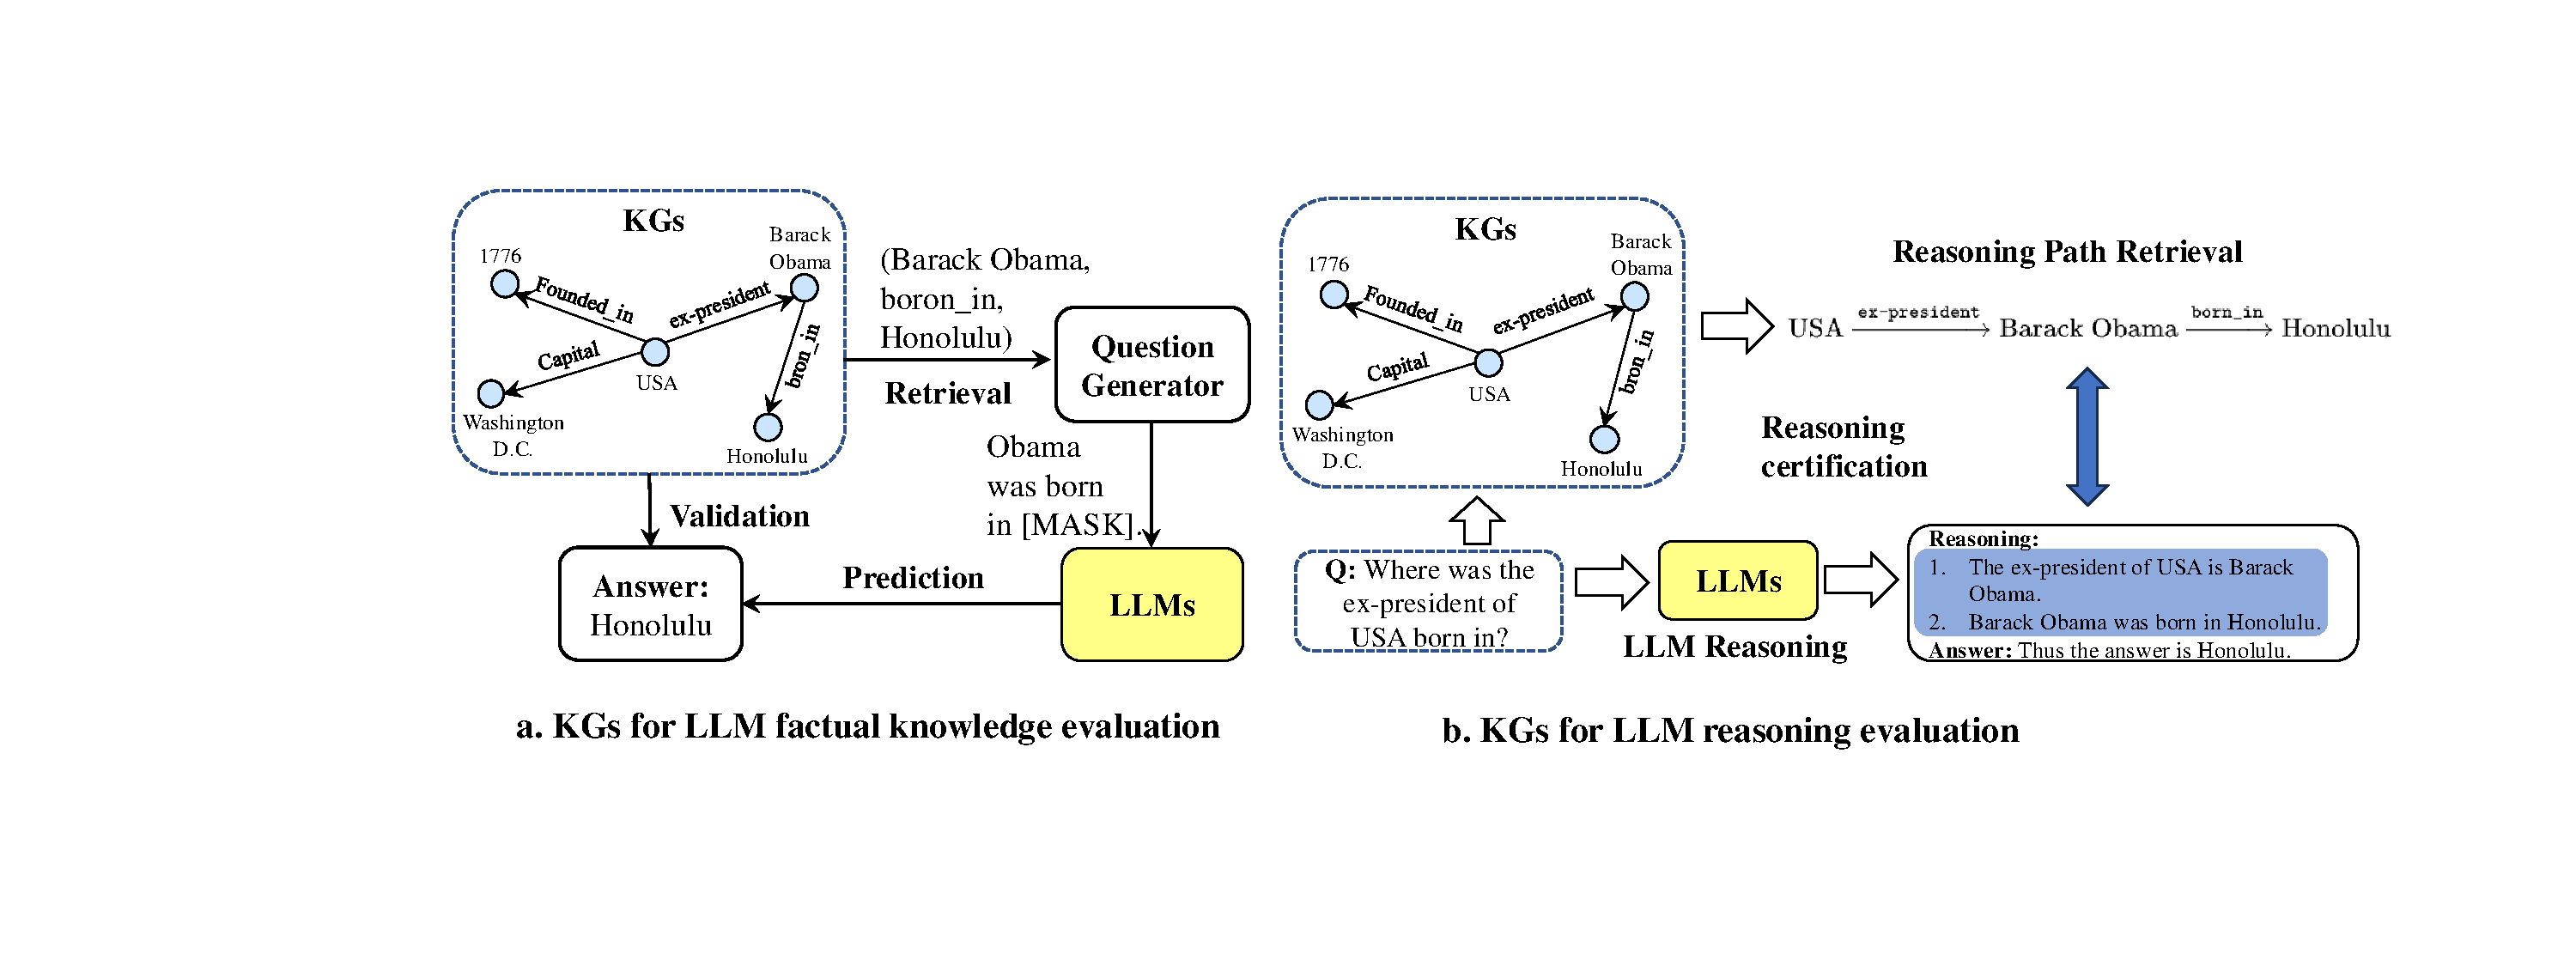
\includegraphics[width=1\columnwidth]{submissions/CarlYang2024/figures/reflecting.pdf}
    \end{center}
    % \vspace{-3mm}
    \caption{The illustration of LLM reflection with KGs. (a) The evaluation of the factual knowledge inside LLMs. (b) The evaluation of the reaosning process of LLMs with KGs.}
    \label{fig:reflecting}
    % \vspace{-5mm}
\end{figure}